%%%%%%%%%%%%%%%%%%%%%%%%%%%%%%%%%%%%%%%%%
% a0poster Landscape Poster - REVAMPED STYLE
% Original Template from: http://www.LaTeXTemplates.com
%%%%%%%%%%%%%%%%%%%%%%%%%%%%%%%%%%%%%%%%%

%----------------------------------------------------------------------------------------
%   PACKAGES AND OTHER DOCUMENT CONFIGURATIONS
%----------------------------------------------------------------------------------------

\documentclass[a0,landscape]{config/poster/a0poster}
\usepackage{config/poster/a0size}

% Core Packages
\usepackage{multicol} % For multiple columns
\usepackage[svgnames]{xcolor} % For custom colors
\usepackage{times} % Use the times font
\usepackage{graphicx} % For including images
\usepackage{booktabs} % For professional tables
\usepackage[font=small,labelfont=bf]{caption} % For figure/table captions
\usepackage{amsfonts, amsmath, amsthm, amssymb} % Math packages
\usepackage[style=ieee]{biblatex} % IEEE style citations

% Styling Packages
\usepackage[most]{tcolorbox} % For creating colored boxes (headers)

\hyphenpenalty=100000
\tolerance=10000

%----------------------------------------------------------------------------------------
%   DOCUMENT CONFIGURATION
%----------------------------------------------------------------------------------------

% Layout settings
\columnsep=80pt % Space between columns
%\columnseprule=3pt % Remove the vertical line for a cleaner look

% Set graphic path
\graphicspath{{./}{resources/chapter-4/}} % Location of the graphics files

% Bibliography resources
\addbibresource{config/paper/IEEEabrv.bib}
\addbibresource{references.bib}

% Custom Colors and Commands
\definecolor{IEEEblue}{rgb}{0.0, 0.21, 0.42} % Define a standard blue for branding

% Command for creating a styled section header
\newcommand{\postersection}[1]{%
  \begin{tcolorbox}[
    colback=IEEEblue,
    colframe=IEEEblue,
    fonttitle=\bfseries,
    coltext=white,
    sharp corners,
    boxrule=0pt,
    top=4pt,
    bottom=4pt,
    halign=center
  ]
    \large #1
  \end{tcolorbox}%
}

%----------------------------------------------------------------------------------------

\begin{document}

%----------------------------------------------------------------------------------------
%   POSTER HEADER 
%----------------------------------------------------------------------------------------

\begin{minipage}[c]{0.8\linewidth}
    \veryHuge \textbf{Large-Scale Event Ticket System Optimization with Distributed Relational Database and Transaction Processing Flow Control} \\[1.5cm]
    \LARGE {Akbar Maulana Ridho} \\
    \Large {13521093@std.stei.itb.ac.id} \\
    \Large {Teknik Informatika, Institut Teknologi Bandung}
\end{minipage}

\vspace{1cm} % Whitespace between header and content

%----------------------------------------------------------------------------------------
%   POSTER BODY
%----------------------------------------------------------------------------------------

\begin{multicols}{4} % Use 4 columns for the body

    %----------------------------------------------------------------------------------------
    %   ABSTRACT
    %----------------------------------------------------------------------------------------

    \postersection{Abstract}
    \begin{quote}
        High-demand event ticketing systems require high throughput and stability under extreme query loads and seat contention. This paper investigates database and application-level optimizations to address these challenges. We evaluate the performance of a traditional PostgreSQL cluster against distributed SQL databases, specifically CitusData and YugabyteDB, for scaling transaction rates. Additionally, we introduce an asynchronous, concurrency-limited order processing flow control scheme designed to reduce database strain by rejecting invalid requests early. Under load tests with 10,000 to 15,000 virtual users, the baseline PostgreSQL cluster demonstrated superior performance with the lowest latency and most efficient resource utilization. In contrast, CitusData showed acceptable but higher latency, while YugabyteDB exhibited poor performance and an unacceptable failure rate. The flow control mechanism, when applied to the PostgreSQL cluster, proved highly effective, significantly reducing database load by pre-emptively filtering requests for unavailable tickets. Our findings suggest that for this specific high-contention workload, a well-tuned monolithic relational database combined with an intelligent application-level flow control strategy provides a more robust and efficient solution than the tested distributed database alternatives.
    \end{quote}

    %----------------------------------------------------------------------------------------
    %   INTRODUCTION
    %----------------------------------------------------------------------------------------

    \postersection{Introduction}
    Online ticket sales for major events present immense technical challenges. High-profile sales, like Taylor Swift's "The Eras Tour," have seen system failures due to overwhelming demand, where millions of users attempt to buy tickets simultaneously \cite{swiftTicketmaster}. This highlights a critical need for systems that can handle extreme, sudden spikes in traffic without failing.

    Ticketing systems face a unique load profile:
    \begin{itemize}
        \item \textbf{Exponential User Arrival:} A massive number of users access the system in a very short window.
        \item \textbf{High Read/Write Load:} Users constantly check for available tickets (reads) while simultaneously trying to purchase them (writes).
        \item \textbf{Extreme Resource Contention:} Many users compete for the exact same limited resources (seats).
    \end{itemize}
    This research investigates various architectural solutions to build a reliable, high-performance ticketing system capable of withstanding these conditions.

    %----------------------------------------------------------------------------------------
    %   OBJECTIVES
    %----------------------------------------------------------------------------------------

    \postersection{Main Objectives}
    This study aims to formulate an optimal and reliable solution for large-scale ticket sales systems by focusing on four key challenges:
    \begin{enumerate}
        \item \textbf{Increase Transaction Throughput:} Evaluate and compare different database architectures (standard vs. distributed) to scale write operations effectively.
        \item \textbf{Optimize Read Operations:} Design and test a multi-layered caching strategy to handle high-volume queries for ticket availability.
        \item \textbf{Ensure Data Integrity:} Implement robust mechanisms within the database to prevent critical errors like double-booking under high concurrency.
        \item \textbf{Maintain System Stability:} Develop and assess an application-level order processing flow control mechanism to manage request spikes and prevent system overload.
    \end{enumerate}

    %----------------------------------------------------------------------------------------
    %   MATERIALS AND METHODS
    %----------------------------------------------------------------------------------------

    \postersection{Methods and Materials}
    \subsection*{Architectures and Technologies}
    We compared three PostgreSQL-compatible database architectures:
    \begin{itemize}
        \item \textbf{PostgreSQL Cluster:} A standard primary-replica setup serving as the performance baseline.
        \item \textbf{CitusData:} A PostgreSQL extension that creates a distributed, coordinator-worker database architecture \cite{citus}.
        \item \textbf{YugabyteDB:} A fully distributed SQL database using the Raft consensus protocol for high availability \cite{yugabyte}.
    \end{itemize}

    To manage the high load, we implemented two key optimization strategies:
    \begin{itemize}
        \item \textbf{Caching with Redis:} An in-memory Redis cluster was used to cache aggregated data to offload read queries from the main database.
        \item \textbf{Flow Control with RabbitMQ:} An asynchronous order processing system was designed using a RabbitMQ message queue to control the rate of requests hitting the database.
    \end{itemize}

    \subsection*{Testing Methodology}
    We used the K6 load testing tool to simulate 10,000-15,000 virtual users. Two main scenarios were tested:
    \begin{enumerate}
        \item \textbf{Sustained Load Test:} A constant high number of users for 10-15 minutes to measure stability and throughput.
        \item \textbf{Ticket Scramble (Spike Test):} A massive initial spike in users to test the system's response to a sudden "ticket drop."
    \end{enumerate}
    Performance was monitored using Prometheus and Grafana.

    %----------------------------------------------------------------------------------------
    %   RESULTS 
    %----------------------------------------------------------------------------------------

    \postersection{Results}
    \subsection*{Database Performance}
    The monolithic PostgreSQL cluster significantly outperformed the distributed databases. It provided the highest throughput at the lowest latency and resource cost. CitusData was acceptable but had ~2x higher latency. YugabyteDB performed poorly, with high instability, >4x latency, and excessive resource usage.

    \begin{center}\vspace{0.5cm}
        \captionof{table}{Overall Performance of Order Processing}
        \begin{tabular}{l l l l}
            \toprule
            \textbf{Metric} & \textbf{PostgreSQL} & \textbf{CitusData} & \textbf{YugabyteDB} \\
            \midrule
            Max Throughput  & 466 rps             & 410 rps            & 216 rps             \\
            Peak CPU Usage  & 8 vCPU              & 10 vCPU            & 19 vCPU             \\
            Peak Memory     & 3.4 GB              & 5 GB               & 36 GB               \\
            Latency (P50)   & 192-382 ms          & 496-650 ms         & 854-10k ms          \\
            \bottomrule
        \end{tabular}
    \end{center}\vspace{0.5cm}

    \subsection*{Read Optimization and Flow Control}
    Caching aggregated availability in Redis was highly effective, handling 1700 rps at just 2.5-4.5 ms latency.

    The flow control mechanism successfully reduced database load. By rejecting requests for unavailable tickets early, latency for failed bookings dropped from 1-2 seconds to just 50-100 ms.

    \begin{center}\vspace{0.5cm}
        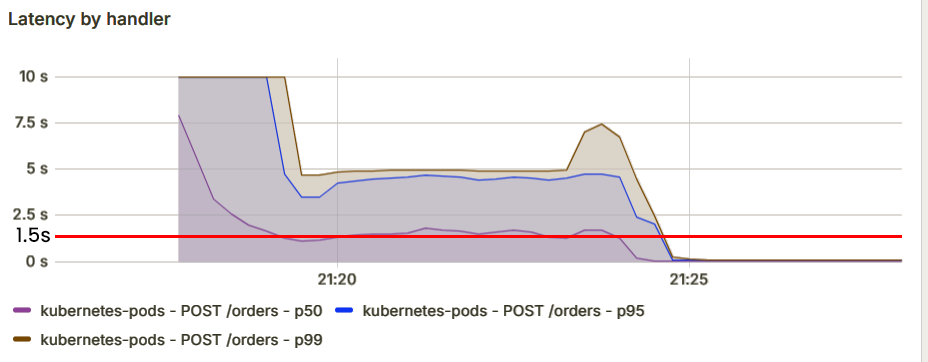
\includegraphics[width=0.9\linewidth]{latency-nofc-pg-stress-0.png}
        \captionof{figure}{High, erratic latency \textbf{without} flow control.}
    \end{center}\vspace{0.5cm}

    \begin{center}\vspace{0.5cm}
        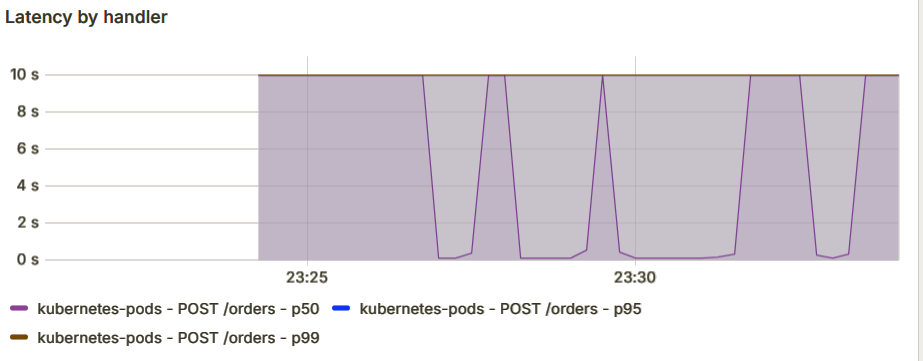
\includegraphics[width=0.9\linewidth]{latency-fc-pg-stress-0.png}
        \captionof{figure}{Lower, more stable latency \textbf{with} flow control.}
    \end{center}\vspace{0.5cm}

    Throughout all high-contention tests, the use of transactional row-level locking (`SELECT ... FOR UPDATE`) proved robust, with zero instances of double-booked seats.

    %----------------------------------------------------------------------------------------
    %   CONCLUSIONS
    %----------------------------------------------------------------------------------------

    \postersection{Conclusions}
    \begin{itemize}
        \item For high-contention transactional workloads, a well-tuned \textbf{monolithic PostgreSQL database offers superior performance} and efficiency compared to the tested distributed solutions.
        \item The overhead of coordination in CitusData and YugabyteDB outweighed their scaling benefits for this specific use case.
        \item \textbf{Flow control, especially early request rejection}, is a critical strategy for maintaining system stability during traffic spikes.
        \item Offloading aggregate read queries to an in-memory store like \textbf{Redis is highly effective}.
    \end{itemize}

    %----------------------------------------------------------------------------------------
    %   FUTURE WORK
    %----------------------------------------------------------------------------------------

    \postersection{Future Work}
    Future work should focus on:
    \begin{enumerate}
        \item Exploring more advanced, distributed caching strategies.
        \item Implementing a lower-latency queueing mechanism to reduce overhead.
        \item Testing the architecture under extreme loads (>100,000 VUs) to find the breaking point of the monolithic setup.
        \item Separating database connection pools for read and write operations.
    \end{enumerate}

    \postersection{Acknowledgements}
    The author thanks his supervisor, Achmad Imam Kistijantoro, S.T., M.Sc., Ph.D., and Dr.techn. Saiful Akbar, S.T., M.T., for their invaluable guidance. Gratitude is also extended to the academic staff of Informatics Engineering at ITB.

    %----------------------------------------------------------------------------------------
    %   REFERENCES
    %----------------------------------------------------------------------------------------

    \postersection{References}
    \printbibliography[heading=none]

\end{multicols}
\end{document}